\documentclass[tikz,border=4pt]{standalone}
\usepackage[T1]{fontenc}
\usetikzlibrary{positioning,arrows.meta,calc}

% two semantic accents only: agent / oracle
\definecolor{agentC}{RGB}{200,98,20}
\definecolor{oracleC}{RGB}{93,58,155}
\definecolor{boxg}{RGB}{245,245,247}
\definecolor{edgeg}{RGB}{120,120,128}
\definecolor{stress}{RGB}{90,90,98}
\definecolor{lane}{RGB}{215,215,220}

\begin{document}
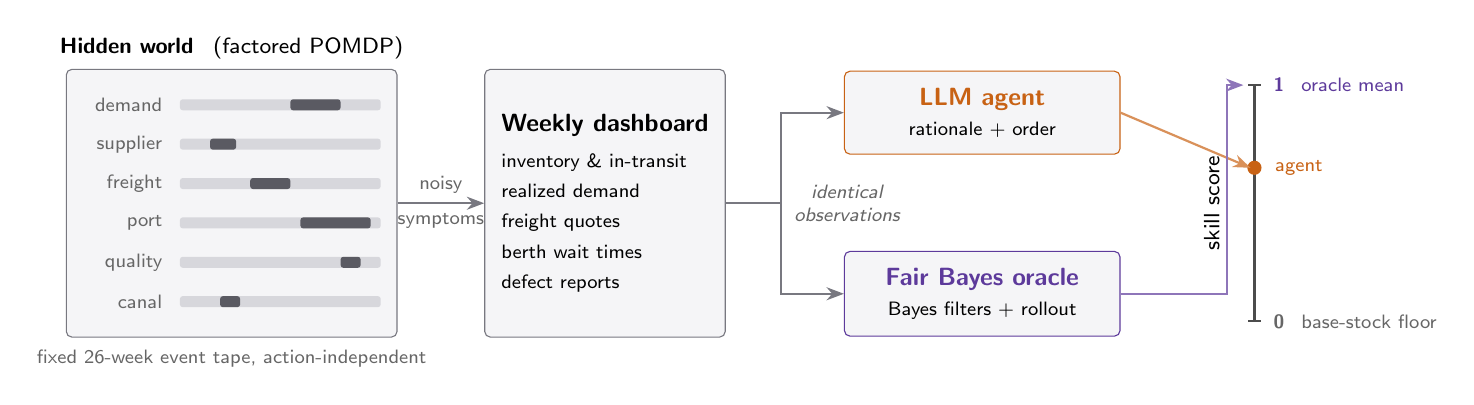
\begin{tikzpicture}[
  font=\small\sffamily,
  box/.style={draw=edgeg, fill=boxg, rounded corners=2pt, inner sep=6pt, align=center},
  lbl/.style={font=\footnotesize\sffamily},
  tiny/.style={font=\scriptsize\sffamily, color=black!60},
  arr/.style={-{Stealth[length=2.2mm]}, thick, color=edgeg},
]

% ---------- Hidden world ----------
\node[box, minimum width=4.2cm, minimum height=3.4cm] (world) at (0,0) {};
\node[lbl, anchor=south] at (world.north) {\textbf{Hidden world} \, (factored POMDP)};
\node[tiny, anchor=north] at ([yshift=-1pt]world.south) {fixed 26-week event tape, action-independent};

% six factor lanes with stress segments
\foreach [count=\i] \name/\sa/\sb in {
    demand/0.55/0.80, supplier/0.15/0.28, freight/0.35/0.55,
    port/0.60/0.95, quality/0.80/0.90, canal/0.20/0.30}{
  \pgfmathsetmacro{\y}{1.25-(\i-1)*0.5}
  \node[tiny, anchor=east] at ($(world.west)+(1.35,\y)$) {\name};
  \draw[fill=lane, draw=none, rounded corners=1pt]
      ($(world.west)+(1.45,\y-0.07)$) rectangle ($(world.west)+(4.0,\y+0.07)$);
  \draw[fill=stress, draw=none, rounded corners=1pt]
      ($(world.west)+(1.45+\sa*2.55,\y-0.07)$) rectangle ($(world.west)+(1.45+\sb*2.55,\y+0.07)$);
}

% ---------- Observations ----------
\node[box, right=1.1cm of world, minimum height=3.4cm, align=left] (obs)
  {\textbf{Weekly dashboard}\\[2pt]
   \scriptsize inventory \& in-transit\\
   \scriptsize realized demand\\
   \scriptsize freight quotes\\
   \scriptsize berth wait times\\
   \scriptsize defect reports};
\draw[arr] (world) -- node[tiny, above]{noisy} node[tiny, below]{symptoms} (obs);

% ---------- Fork: agent & oracle ----------
\node[box, right=1.5cm of obs.east, yshift=1.15cm, draw=agentC, minimum width=3.5cm] (agent)
  {\textcolor{agentC}{\textbf{LLM agent}}\\ \scriptsize rationale + order};
\node[box, right=1.5cm of obs.east, yshift=-1.15cm, draw=oracleC, minimum width=3.5cm] (oracle)
  {\textcolor{oracleC}{\textbf{Fair Bayes oracle}}\\ \scriptsize Bayes filters + rollout};

\coordinate (fork) at ($(obs.east)+(0.7,0)$);
\draw[thick, color=edgeg] (obs.east) -- (fork);
\draw[arr] (fork) |- (agent.west);
\draw[arr] (fork) |- (oracle.west);
\node[tiny, align=center] at ($(fork)+(0.85,0)$) {\emph{identical}\\ \emph{observations}};

% ---------- Skill scale ----------
\coordinate (sc) at ($(agent.east)+(1.7,-1.15)$);
\draw[thick, color=black!70] ($(sc)+(0,-1.5)$) -- ($(sc)+(0,1.5)$);
\foreach \y/\t in {-1.5/0, 1.5/1}{
  \draw[thick, color=black!70] ($(sc)+(-0.08,\y)$) -- ($(sc)+(0.08,\y)$);
}
\node[tiny, anchor=west] at ($(sc)+(0.12,-1.5)$) {\textbf{0} \, base-stock floor};
\node[tiny, anchor=west, color=oracleC] at ($(sc)+(0.12,1.5)$) {\textbf{1} \, oracle mean};
\node[lbl, anchor=south, rotate=90] at ($(sc)+(-0.32,0)$) {skill score};

% agent marker on scale
\fill[agentC] ($(sc)+(0,0.45)$) circle (0.09);
\node[tiny, anchor=west, color=agentC] at ($(sc)+(0.14,0.45)$) {agent};

\draw[arr, color=agentC!70] (agent.east) -- ($(sc)+(-0.05,0.45)$);
\draw[arr, color=oracleC!70] (oracle.east) -| ($(sc)+(-0.35,1.5)$) -- ($(sc)+(-0.14,1.5)$);

\end{tikzpicture}
\end{document}
